\section{There and back again}
\label{sec:prequel}
In this section we will try to shed some light on the preliminary work that was done before we ended up on the path that lead to our project. It consists of two parts. The first will be a summary of our pre-project and the second on our early work with Voldemort. 
This section can be skipped for most readers as it is not the most relevant for the thesis, but have been included because it was how the project started.

\subsection{Energy efficiency of a Raspberry Pi cluster used for searching}
Our pre-project was split into three parts. Building a cluster of Raspberry Pis, building a search engine and then measure performance and power efficiency of our cluster compared to a Core i5 Macbook Pro. During the build we constructed our own power supply and built the frame holding the cluster along with network equipment. The search engine was written in C to be as fast as possible. We used an existing python program to create an index over a corpus of text documents, and used tf-idf for scoring results. Through our performance testing we found that even though the Pis require a lot less energy to run, they are unable to keep up with modern hardware in a task so bound by CPU. It is worth mentioning that our entire index fit into memory, so a more disk bound application could have seen very different results. We however feel this is unlikely, due to the disk controller on the Pi being very slow and USB based with no DMA, so it requires CPU cycles to do any operation.

\begin{figure}[h]
    \centering
    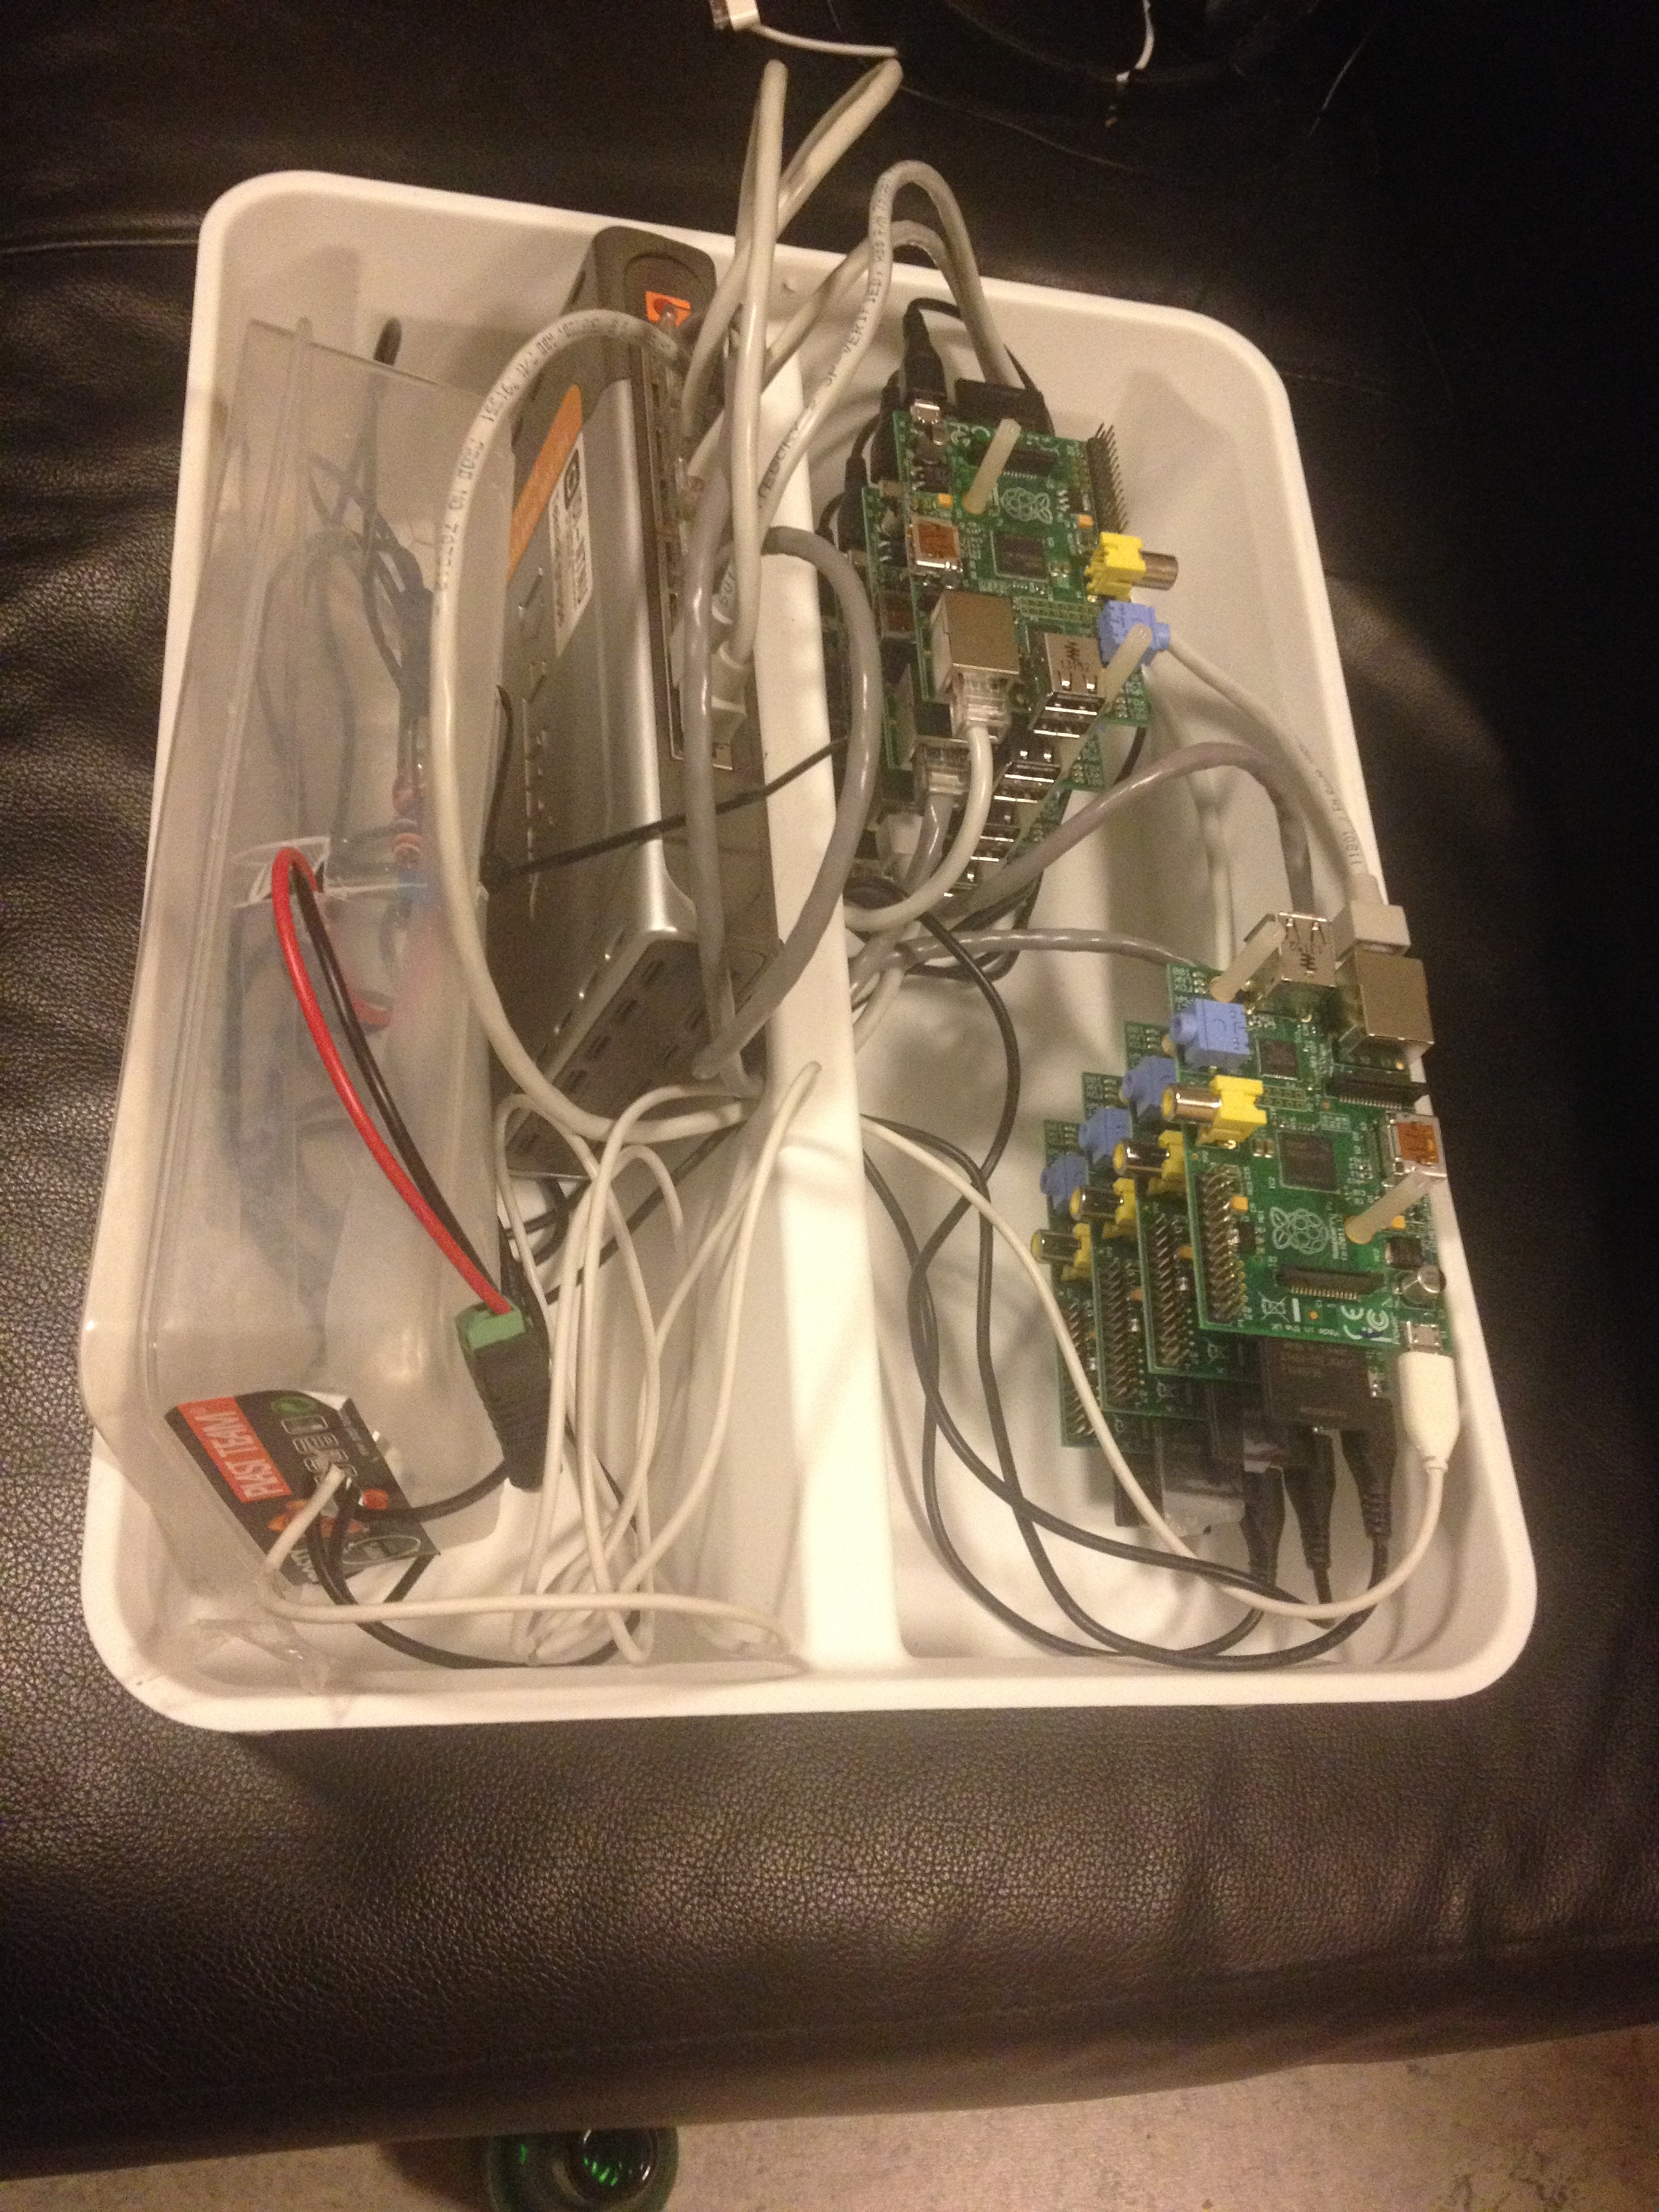
\includegraphics[width=0.5\textwidth]{introduction/figures/cluster_beautiful}
    \caption{The Raspberry Pi cluster}
    \label{fig:cluster}
\end{figure}

\subsection*{Early work with Raspberry Pis and Voldemort}
In the early days of our project we were planning to use our Raspberry Pi cluster to host a Voldemort service. However the limited memory of 512MB quickly turned out to be a problem. The Pis could run Voldemort without any problems until some of the background data exchange processes started and killed the JVM. After some debugging we determined that memory was a serious issue, and abandoned the idea of running Voldemort on our Pis. They do not have enough RAM for any practical uses of the software.

To try out how much more powerful hardware you need to run a cluster based on Voldemort, we decided to give virtual machines a try. We used an older Mac mini (mid 2010) with a 2.4 Ghz Core 2 Duo processor and 8 GB of RAM, and created 4 virtual machines using VMware Fusion. They were all setup to run Arch Linux with 1 GB memory allocated. Initial tests quickly showed that these had no issues with running out of memory. After querying the institute for a proper solution we were allowed access to 4 virtual machines running on a server within the institute. These servers were running on a Intel(R) Xeon(R) CPU E5-2650 @ 2.00GHz host, with each VM granted 1 GB RAM. The network to these machines were however clogged by several 100mbit links, so we could not get much performance from them, and decided to work more locally.

\subsection{Post mortem}
In our pre-project we built a search engine and ran it on a cluster composed of 8 Raspberry Pis. In this project we wanted to work with a more developed distributed system and explore what possibilities existed for further work, but the typical software packages were unable to run reliably on a small system like the Pi. The main problem was the OS running out of memory.

